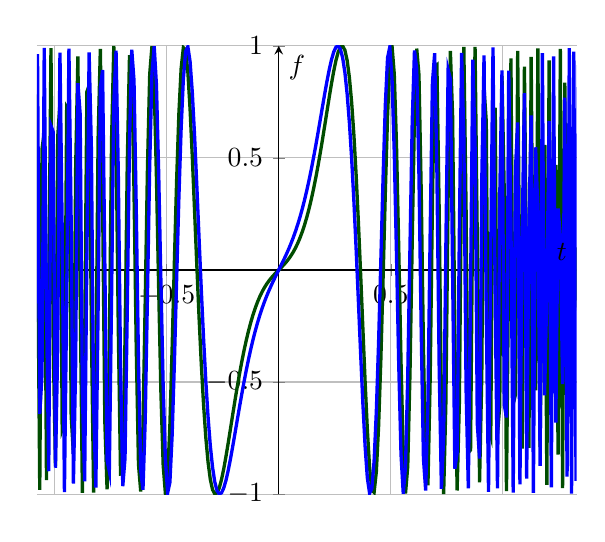
\begin{tikzpicture}
	\begin{axis}[axis lines=middle, axis equal, grid=both, xmin = 0, xmax = 0.25, ymin = -1, ymax = 1, xlabel = $t$, ylabel = $\operatorname{f}$]
		\addplot[black!70!green, very thick, samples = 1000] {sin(deg(x^2)*deg(x)+deg(x))} node[above, red] at (100, 100) {$f$};
		\addplot[blue, very thick, samples = 1000] {sin(deg(x^2)*deg(x)+deg(2*x))} node[above, red] at (100, 100) {$f$};
	\end{axis}
\end{tikzpicture}